
\chapter{Observable to Study the Underlying Event}
\label{chap:ObservabletoStudytheUnderlyingEvent}

The UE are all the processes not associated with the primary hard scatter in an hadron-hadron collision.

All the process described in the previous section: ISR and FSR, MPI, and BBR and their interactions with color exchanges among them, contribute to the Underlying Event (UE) in the proton-proton collision.

The most of the observable to study the UE are sensible only to the sum of these contributions and not to the single ones so a good description of all this process and their interplay is really important.

\section{Minimum Bias Measurements and Underlying Event topology}

A Minimum Bias (MB) measurement is a collection of inelastic events with a loose event selection. The events are collected requiring the minimal interaction with the detector (the smallest possible bias). The most of the interaction in MB observation are soft, $p_T\lesssim2\ \mathrm{GeV}$. The study of the UE require at least one hard scattering ($p_T\gtrsim2\ \mathrm{GeV}$) presence.
 
To study the UE the topological structure of an hadron hadron collision is used. On an event-by-event analysis the direction of the leading object is used to define regions in the $\eta-\phi$ space. Where $\eta$ is the pseudorapidity defined as $\eta=-\log{\tan\left(\frac{\theta}{2}\right)}$, while $\phi$ is the azimuthal angle in the $x-y$ plane. 
The last one is defined from the direction of the leading object as $\Delta\phi=\phi-\phi_{\text{leading}}$ .

\begin{figure}[!ht]
	\centering
	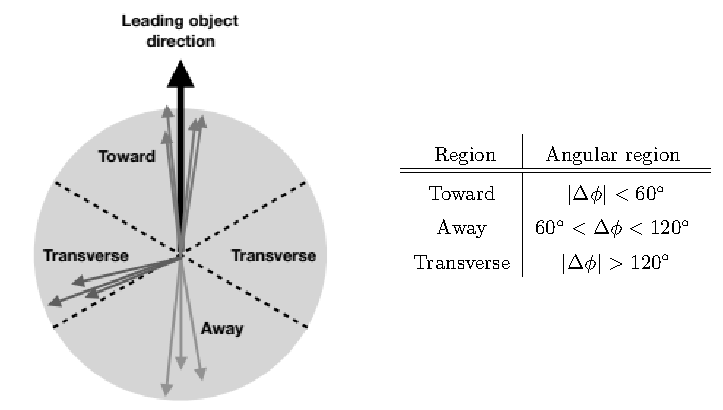
\includegraphics[width=0.8\textwidth]{{img/Regions.pdf}}
	\caption{This figure shows the four regions for the description of the UE on a event-by-event analysis. the angular values are shown in the table. The regions are defined starting from the leading object direction. The toward and away regions contain most of the contribution from the hard scattering (e.g. in a $t\overline{t}$ production event the two quark $t$ are located in these regions); while, the transverse region are the ones in between the twp other regions, these are the most important for the study of the UE.}
	\label{fig:Regions}
\end{figure}


The regions classification is shown in \figRef{fig:Regions}, we have:
\begin{itemize}
	\item \textbf{Toward region}: the region that contains the leading object, this region contains the most of the particle produced by the hard interaction.
	\item \textbf{Away region}: this region contains the objects that recoil against the leading object, also this region contains mostly the particles produced by the hard interaction.
	\item \textbf{Transverse regions}: the two transverse regions are the most sensitive to UE.
\end{itemize}
The transverse regions are also separated in:
\begin{itemize}
	\item[--] \textbf{TransMAX}: This is the transverse region that contains the \textit{maximum} number of charged particles, or scalar $p_T$ sum of charged particles. This regions includes both MPI and hard-process contamination.
	\item[--] \textbf{TransMIN}: is the transverse region that contains the \textit{minimum} number of charged particles, or scalar $p_T$ sum of charged particles. This region is the most  sensitive to MPI effects.
\end{itemize}

The leading object definition depend on the type of event under observation. 

The charged-particle with largest $p_T$ \cite{CMS-PAS-FSQ-15-007}, the dilepton system in Drell-Yan observation \cite{CMS:2012oqb, CMS:2017ngy} or $t\overline{t}$ events \cite{CMS:2018mdd} can all be used as leading object in the analyses for the UE event.


